\documentclass{beamer}
\usepackage{lmodern}
\usetheme{Madrid}
\usepackage{hyperref}
\usepackage{apacite}
\usepackage{verbatim}
\usepackage{xcolor}
% \setbeamertemplate{background}{\tikz[overlay,remember picture]\node[opacity=.2]at (current page.center){\includegraphics[width=7.8cm]{Python.jpg}};}
\usepackage{tikz}
\usepackage{kantlipsum}

\setbeamercolor{normal text}{fg=black}

\begin{document}
\colorlet{beamer@blendedblue}{blue!46!green}
\setbeamercolor{normal text}{fg=black}

\setbeamercolor{frametitle}{fg=white, bg=blue!46!green}
\setbeamercolor*{title}{bg=blue!46!green, fg=white}

\setbeamercolor{section in toc}{fg=black}


\author[Juan C. Correa, Ph.D.]{Juan C. Correa, Ph.D.}
\title[Análisis Estadísticos en Python]{Aprendiendo Python para Análisis Estadísticos}
% \subtitle{A Research Agenda}
	%\subtitle{}
\institute[]{
	\color{blue}\Email  \href{mailto:j.correa.n@gmail.com}{j.correa.n@gmail.com}}
\pgfdeclareimage[height=.7cm]{Python}{Python}
\logo{\pgfuseimage{Python}}
\setbeamertemplate{caption}[numbered]
\date[Mayo 2021]{\textcolor{blue}{\url{https://correajc.com/}}}

%\subject{}
\setbeamercolor{background canvas}{bg=white}
%\setbeamertemplate{navigation symbols}{}

\begin{frame}
	\titlepage
\end{frame}

\begin{frame}
\begin{block}{Objetivo de esta charla}
\vspace{0.3cm}
Introducir los aspectos preliminares de Python para implementar un análisis de regresión simple y múltiple (sin conocer las otras funcionalidades de Python)  \end{block}
\end{frame}

\begin{frame}
\frametitle{Agenda} 
\tableofcontents
\end{frame}



\section{Preliminares}
\begin{frame}{Preliminares}
 \begin{figure}

\includegraphics[width=1\textwidth]{tools.png}
\end{figure}
El primer paso es descargar anaconda navigator \textcolor{blue}{\url{https://www.anaconda.com/products/individual}}
\end{frame}

\begin{frame}{Preliminares}
Anaconda gestiona multiples versiones de Python
sobre la máquina, además de ofrecer una gran colección de librerías comúnmente usadas en data science. Por eso es más práctico trabajar en Python a través de Anaconda en lugar de hacerlo con otras herramientas. 
\begin{figure}

\includegraphics[width=.6\textwidth]{equivalent.png}
 \end{figure}
\end{frame}


\begin{frame}{Preliminares}
Para ingresar a Anaconda, se abre la terminal del sistema operativo y se escribe \texttt{anaconda-navigator} + enter
\begin{figure}
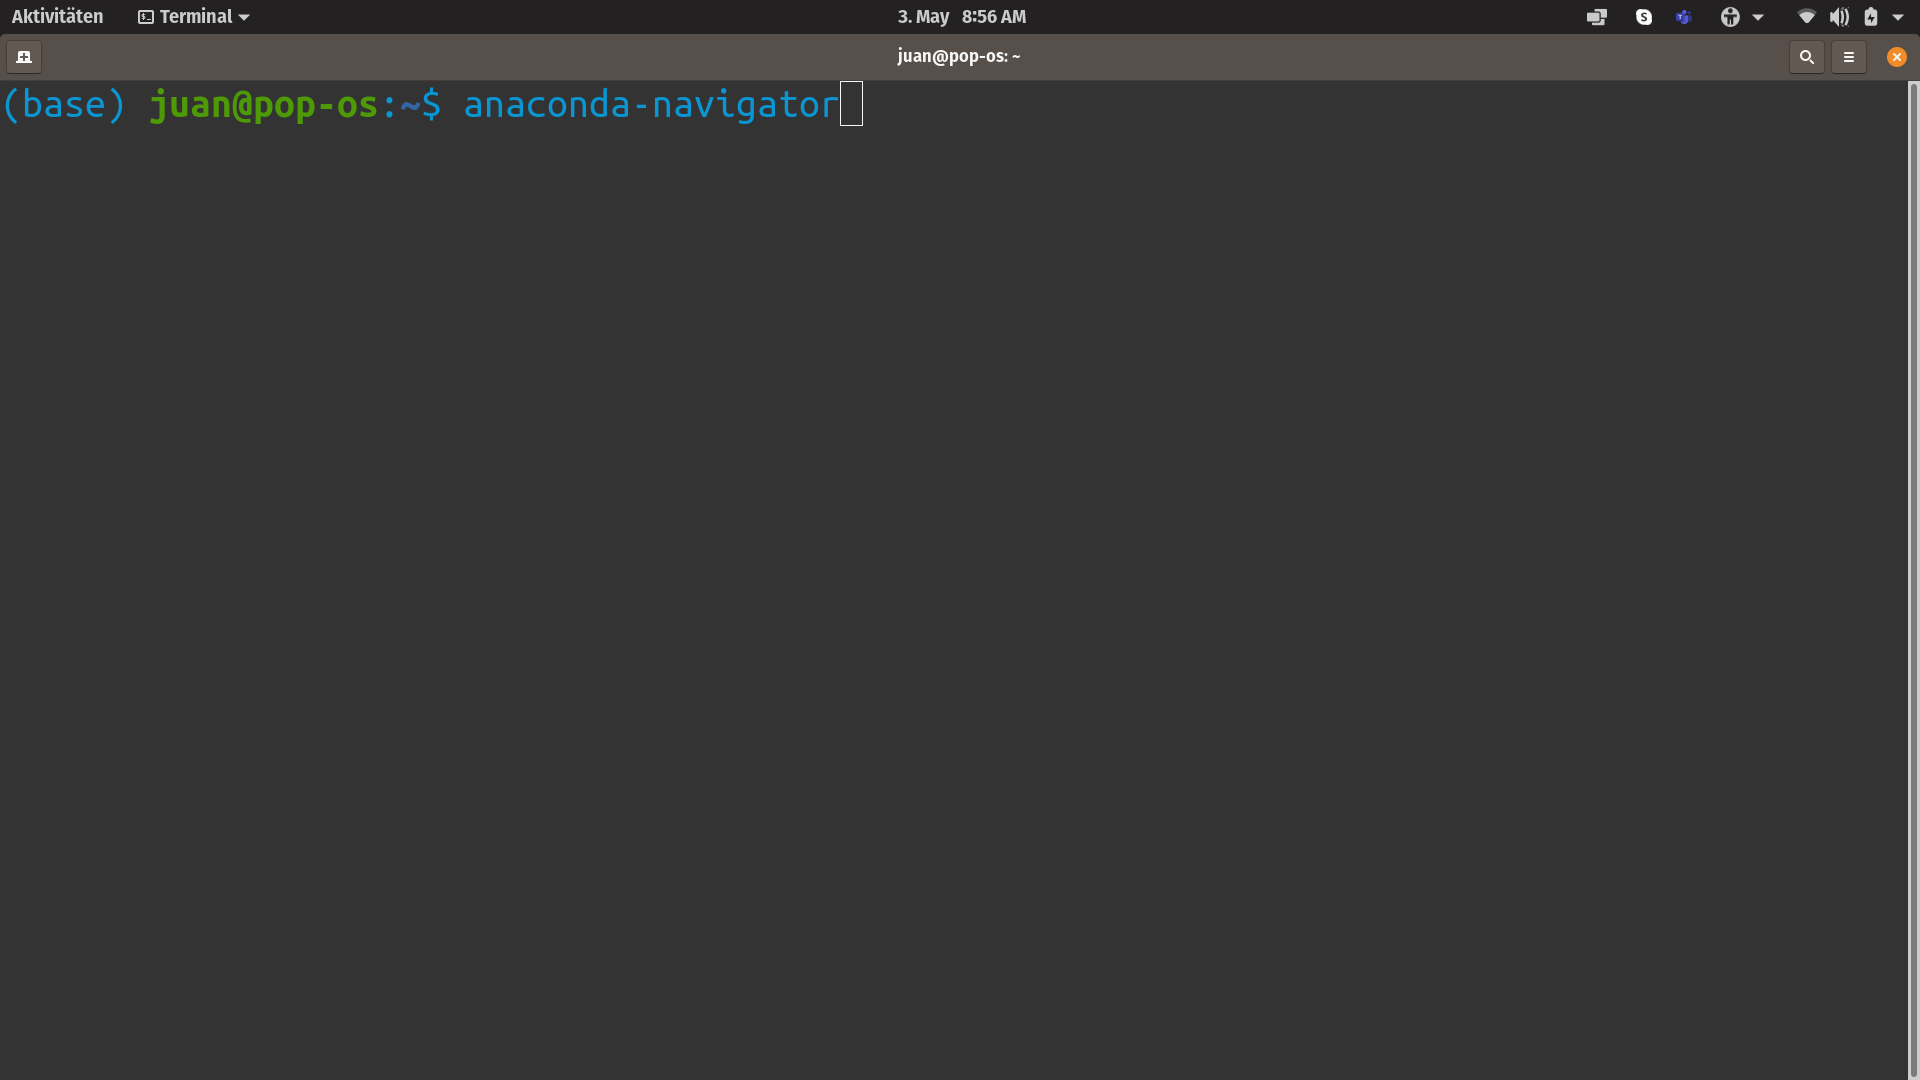
\includegraphics[width=.8\textwidth]{terminal.png}
 \end{figure}
\end{frame}

\begin{frame}{Preliminares}
Los paquetes incluidos en Anaconda son:
\vspace{0.5cm}
\begin{itemize}
\item \textbf{NumPy} Computación Numérica sobre arrays n-dimensionales
\item \textbf{SciPy} Computación Científica
\item \textbf{Matplotlib} Visualización de datos en 2D
\item \textbf{Pandas} Estructuras de datos y análisis de datos estructurados
\item \textbf{Seaborn} Visualización de datos
\item \textbf{Bokeh} Visualización Web Interactiva
\item \textbf{Scikit-Learn} Machine learning y data mining
\item \textbf{NLKT} Procesamiento de Lenguaje Natural
\item \textbf{Jupyter Notebook} App Web para crear cuadernos reproducibles
\item \textbf{R essentials}
\end{itemize}
\end{frame}

\begin{frame}{Preliminares}
\begin{figure}
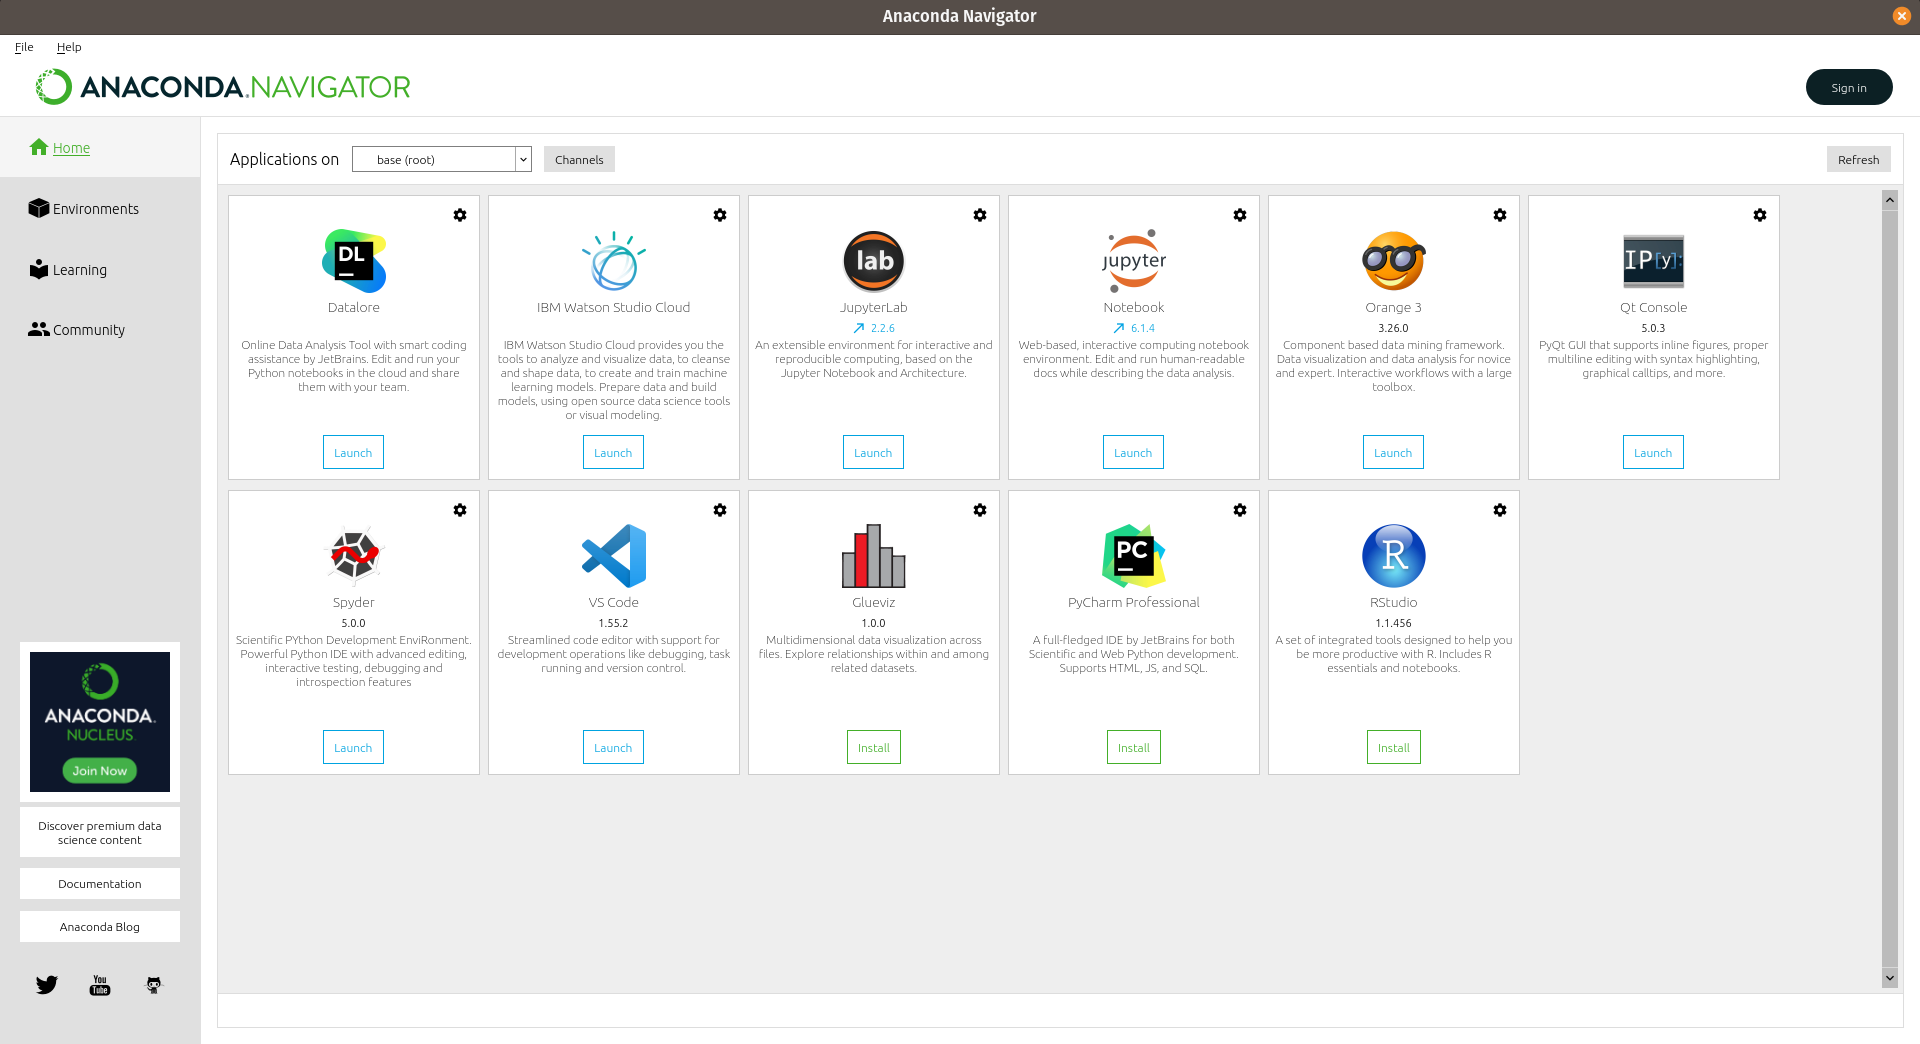
\includegraphics[width=.8\textwidth]{anaconda.png}
 \end{figure}
Interfaz gráfica de Anaconda
\end{frame}

\begin{frame}{Preliminares}
\begin{figure}

\includegraphics[width=.8\textwidth]{Install.png}
 \end{figure}
Para instalar nuevas librerías dentro de Anaconda, basta con hacer clic en ``Environments'' y luego seleccionar el menú \textbf{Not Installed} para escribir a mano derecho el nombre específico de la librería que se quiere instalar.
\end{frame}

\section{Trabajando con Jupyter Notebooks}
\begin{frame}{Trabajando con Jupyter Notebooks}
\begin{figure}
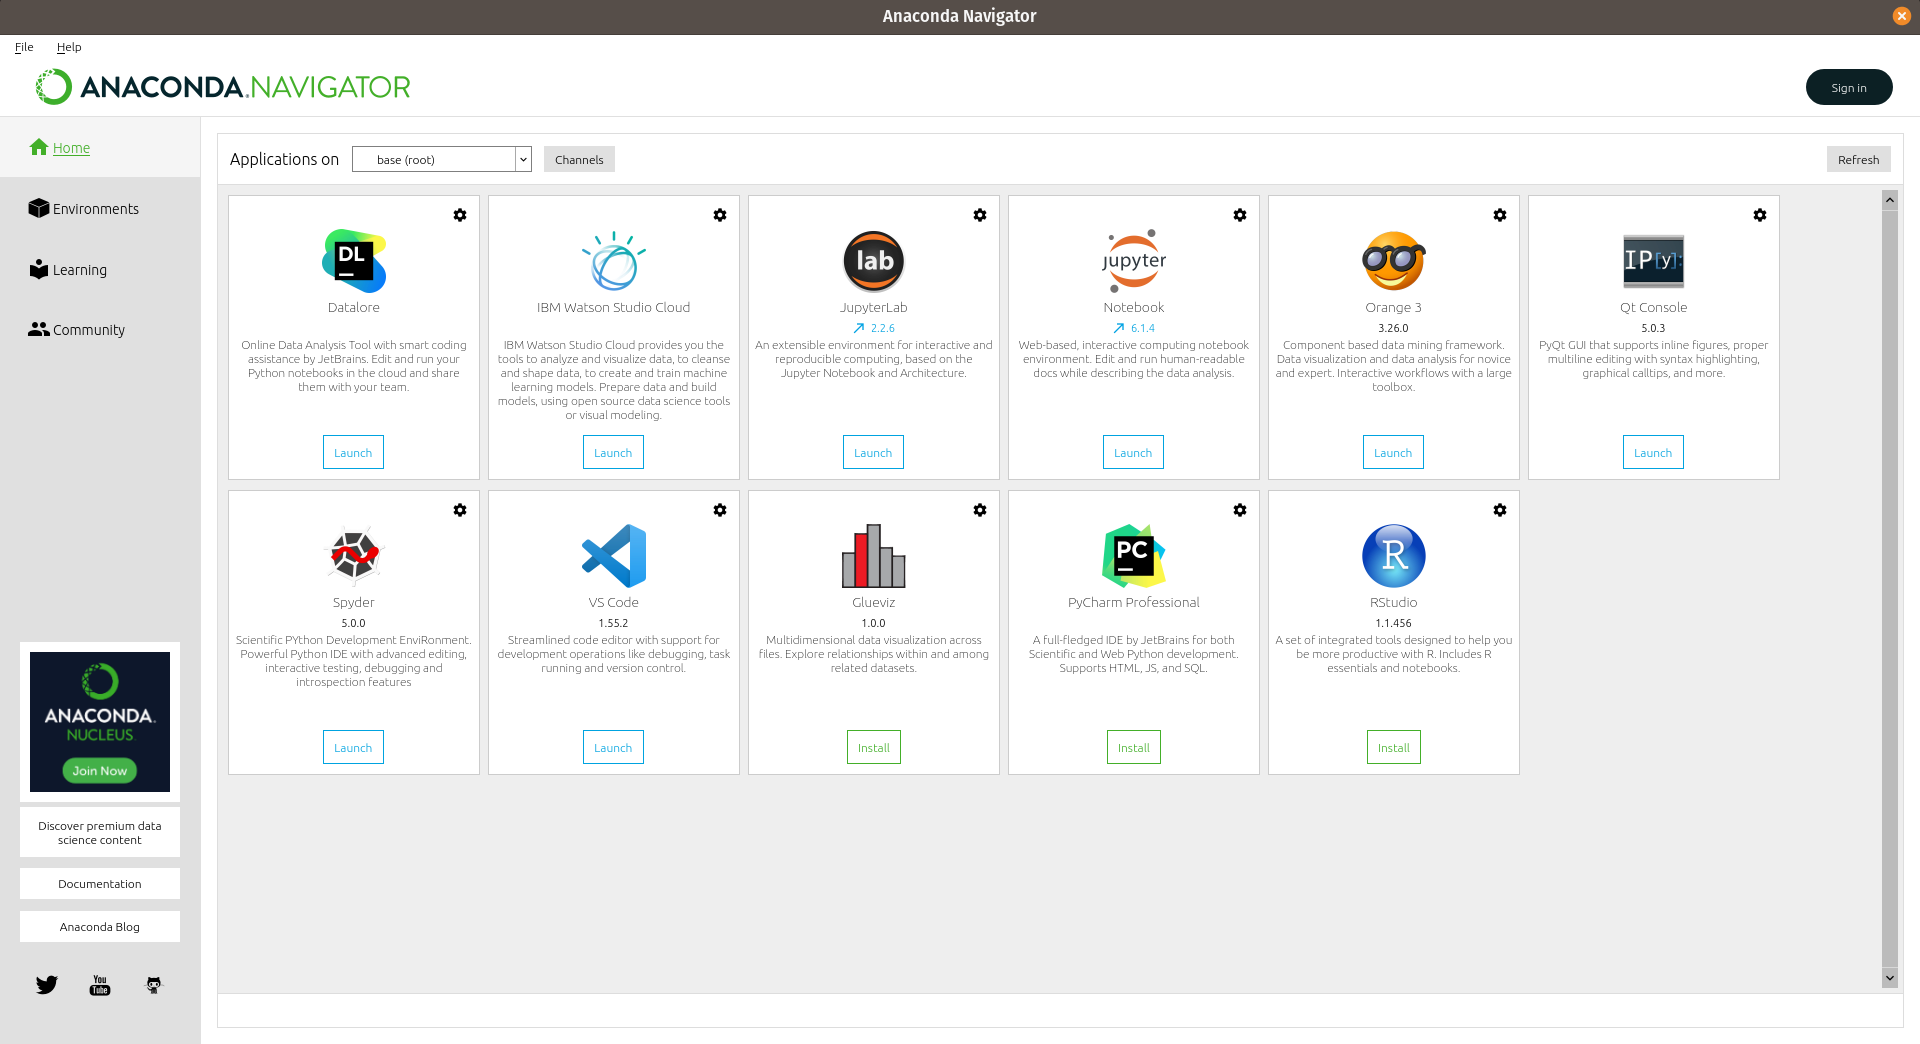
\includegraphics[width=.8\textwidth]{anaconda.png}
 \end{figure}
Clic en \textbf{Launch} dentro del cuadro Jupyter Notebook
\end{frame}


\begin{frame}{Trabajando con Jupyter Notebooks}
\begin{figure}
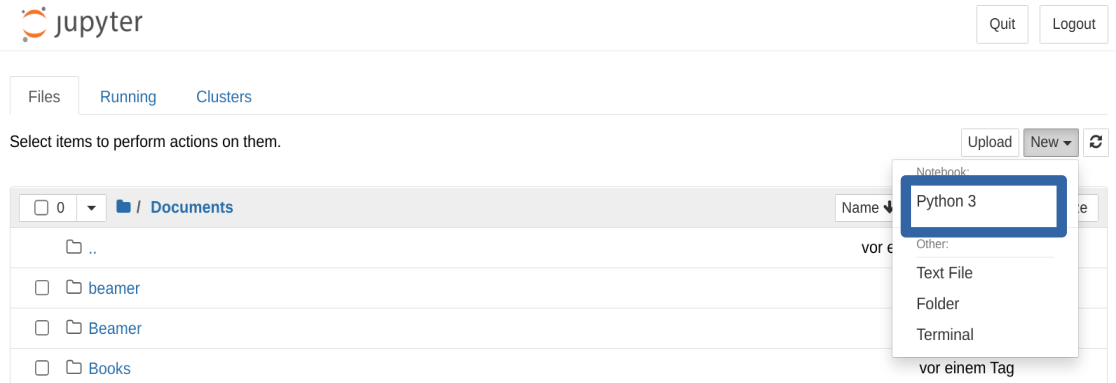
\includegraphics[width=1\textwidth]{jupyter.png}
 \end{figure}
Clic en \textbf{New} y luego en \textbf{Python 3}
\end{frame}

\begin{frame}{Trabajando con Jupyter Notebooks}
\begin{figure}
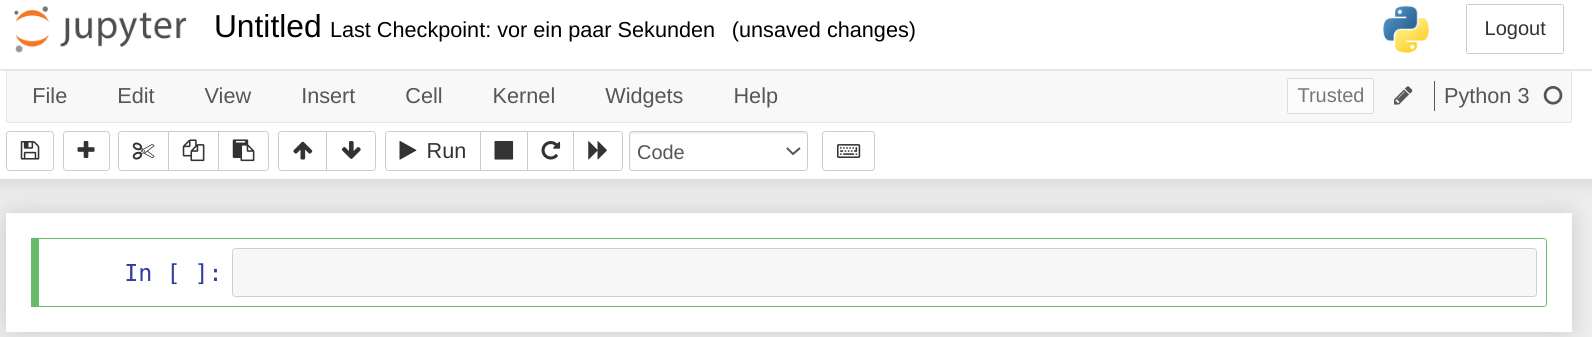
\includegraphics[width=1\textwidth]{JN.png}
\end{figure}
De manera predeterminada, los archivos creados en jupyter notebook tienen el nombre \textbf{Untitled}. Debemos cambiarle el nombre haciendo clic sobre Untitled.
\end{frame}

\begin{frame}{Trabajando con Jupyter Notebooks}
\begin{figure}
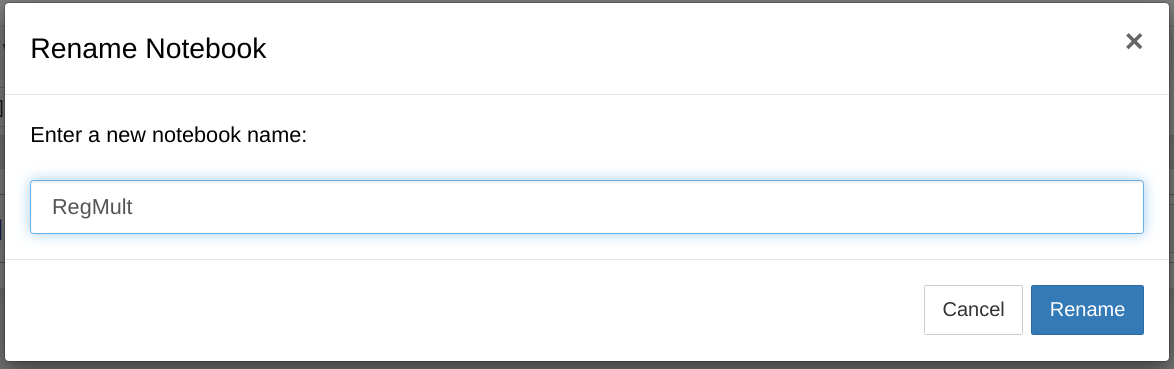
\includegraphics[width=1\textwidth]{rename.png}
\end{figure}
Acá vamos a poner el nombre a nuestro primer Jupyter Notebook como \textbf{RegMult}.
\end{frame}

\begin{frame}{Trabajando con Jupyter Notebooks}
\begin{figure}
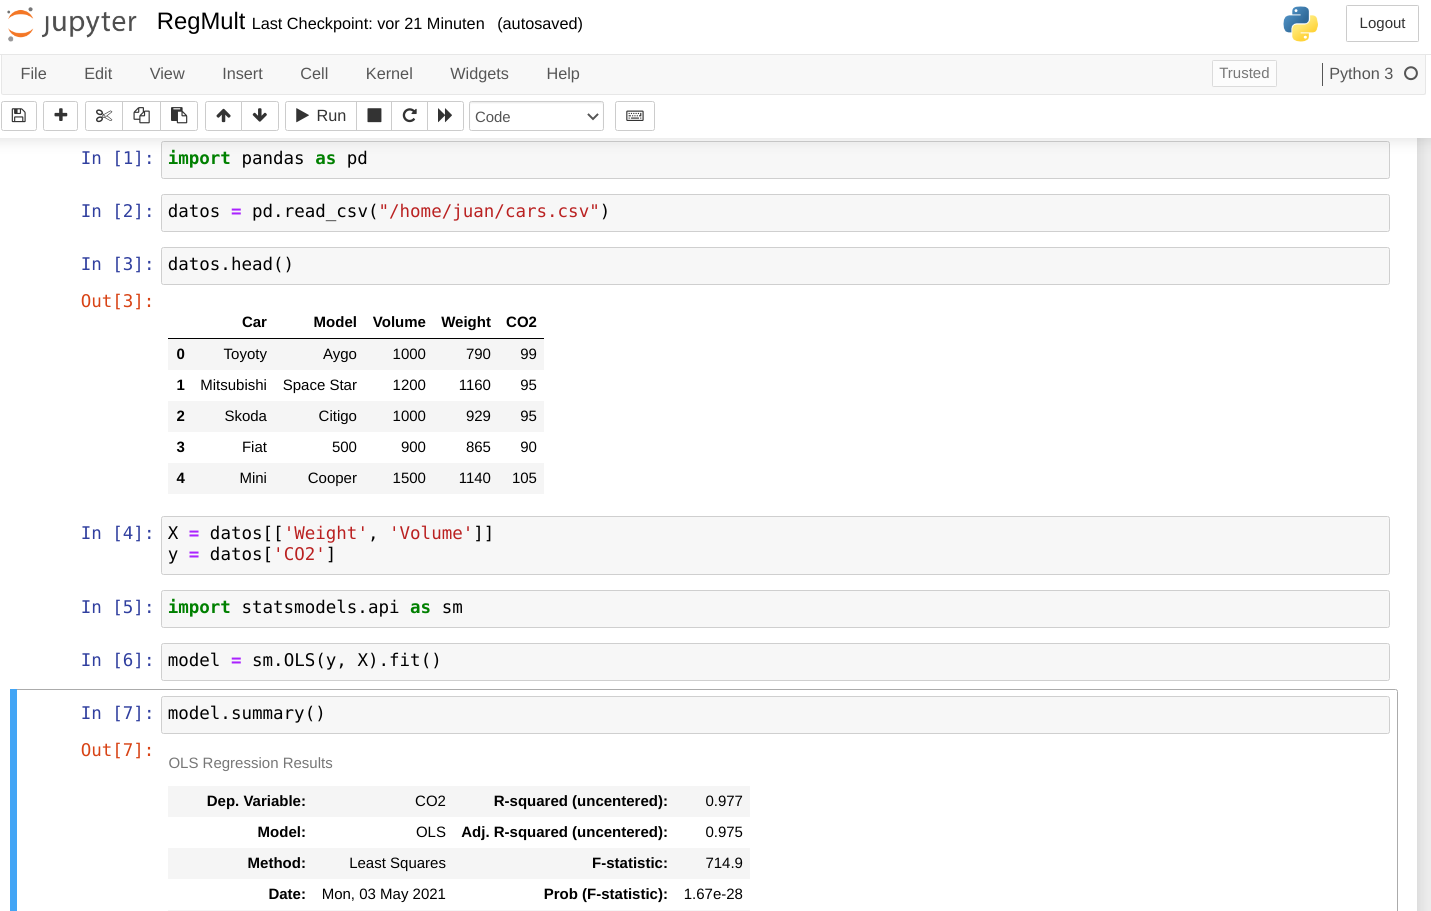
\includegraphics[width=.85\textwidth]{RM.png}
\end{figure}
\end{frame}

\begin{frame}{Trabajando con Jupyter Notebooks}
\begin{figure}
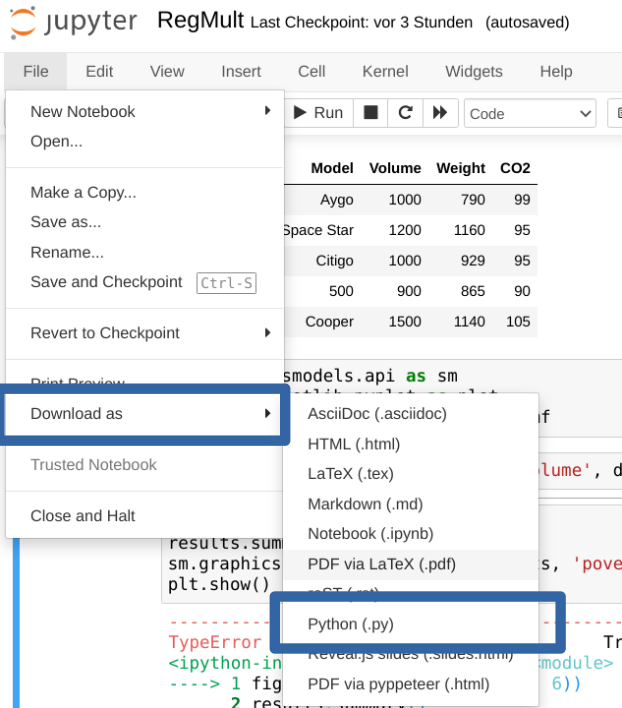
\includegraphics[width=.55\textwidth]{Dsk.png}
\end{figure}
\end{frame}

\section{Trabajando con Spyder}
\begin{frame}{Trabajando con Spyder}
\begin{figure}
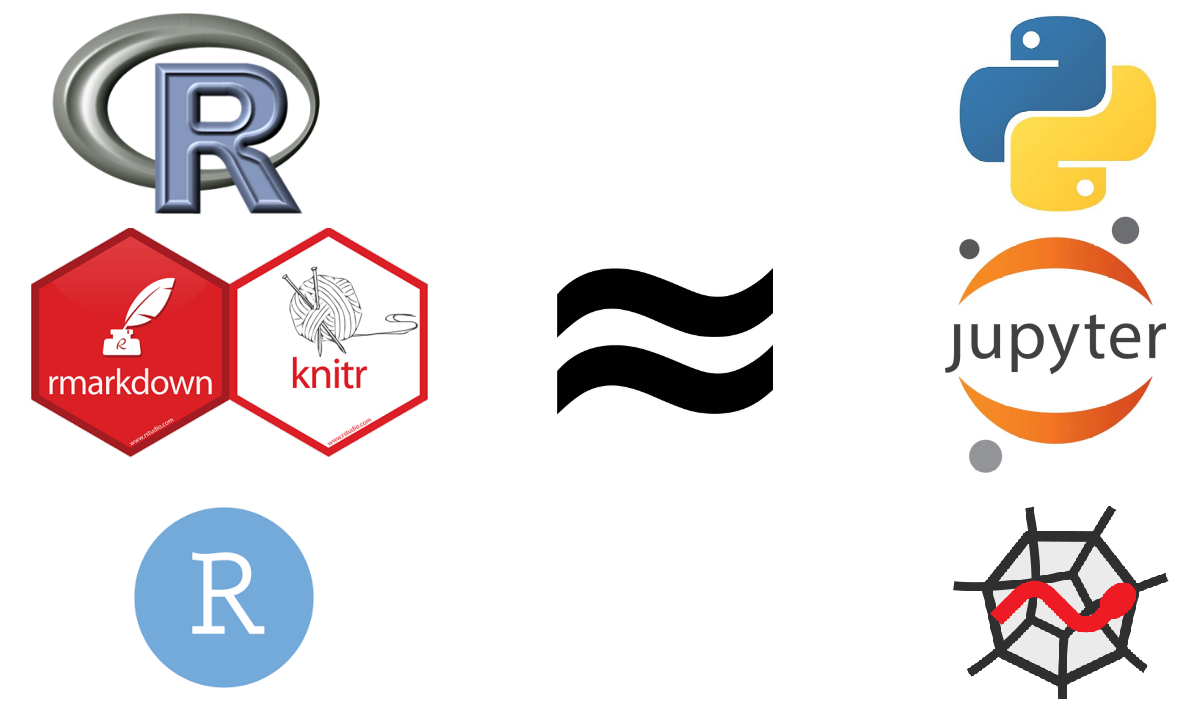
\includegraphics[width=.75\textwidth]{eq.png}
\end{figure}
La apariencia de Spyder es muy similar a la de RStudio 
\end{frame}

\begin{frame}{Trabajando con Spyder}
\begin{figure}
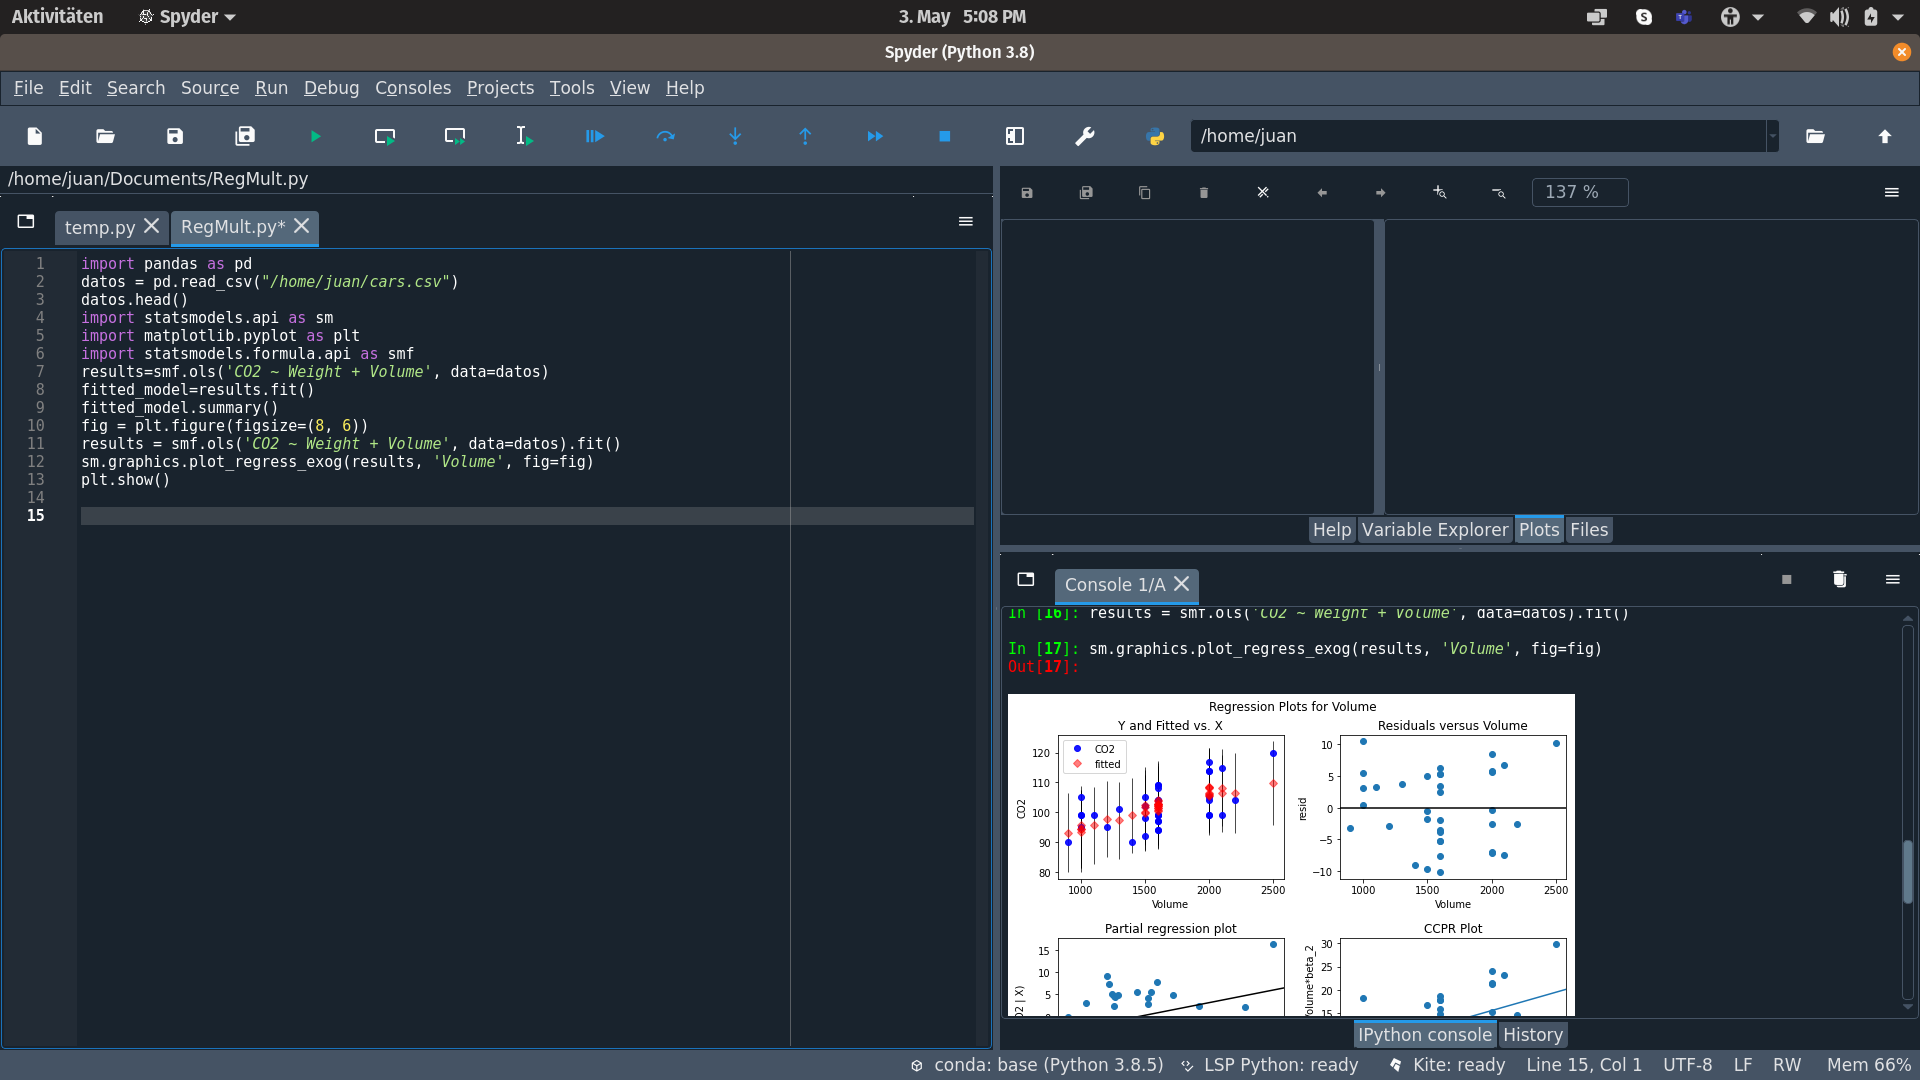
\includegraphics[width=.9\textwidth]{spyder.png}
\end{figure}
Trabajar en Spyder es como elaborar un script en R (archivo .R)
\end{frame}


\begin{frame}{Trabajando con Spyder}
Hay varias semejanzas entre Python y R, desde el punto de vista de las instrucciones (sintaxis) que debemos escribir para que el software realice lo que deseemos.\\
\vspace{0.5cm}
\texttt{\textcolor{magenta}{import} pandas as pd} \\
\texttt{\textcolor{blue}{library}(readr)}\\
\vspace{0.5cm}
\texttt{datos = pd.read\_csv("/home/juan/cars.csv")} \\ \texttt{readr::datos <- read\_csv("/home/juan/cars.csv")}
\end{frame}

\section{Recursos Bibliográficos}
\begin{frame}{Recursos Bibliográficos}
\begin{figure}
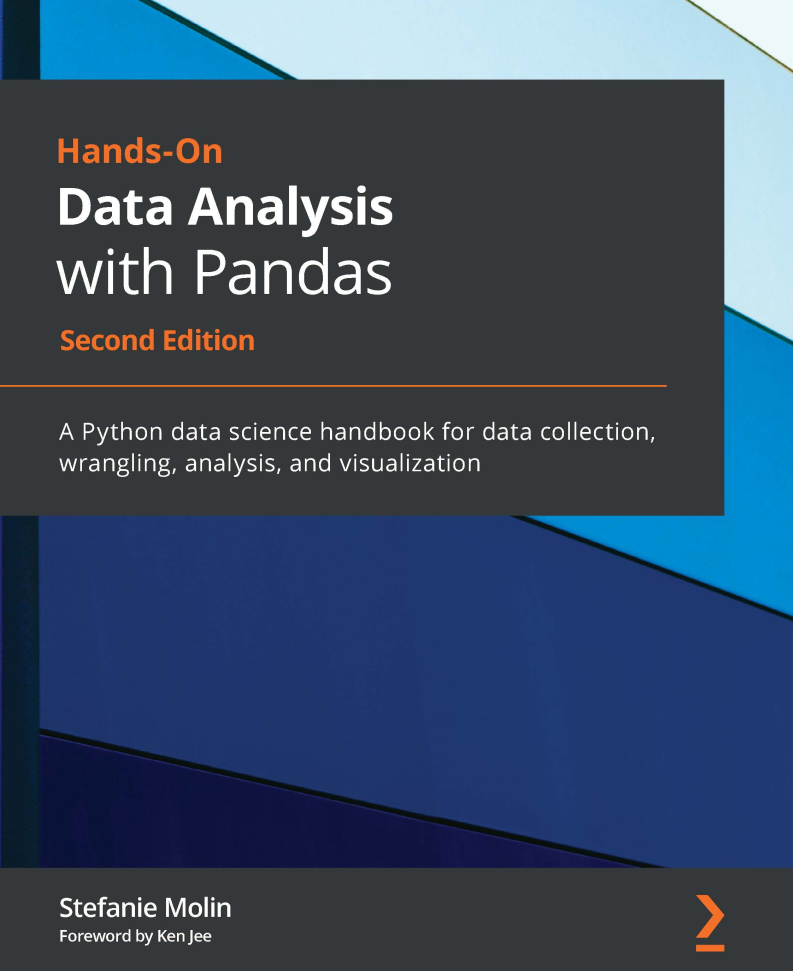
\includegraphics[width=.3\textwidth]{book.png}
\end{figure}
El libro de \citeauthor{Molin2021} \citeyear{Molin2021} es un buen recurso para aprender fundamentos de análisis de datos. Pero su aproximación dista mucho del tipo de estadística aplicada en psicología.
\end{frame}

\begin{frame}{Recursos Bibliográficos}
\begin{figure}
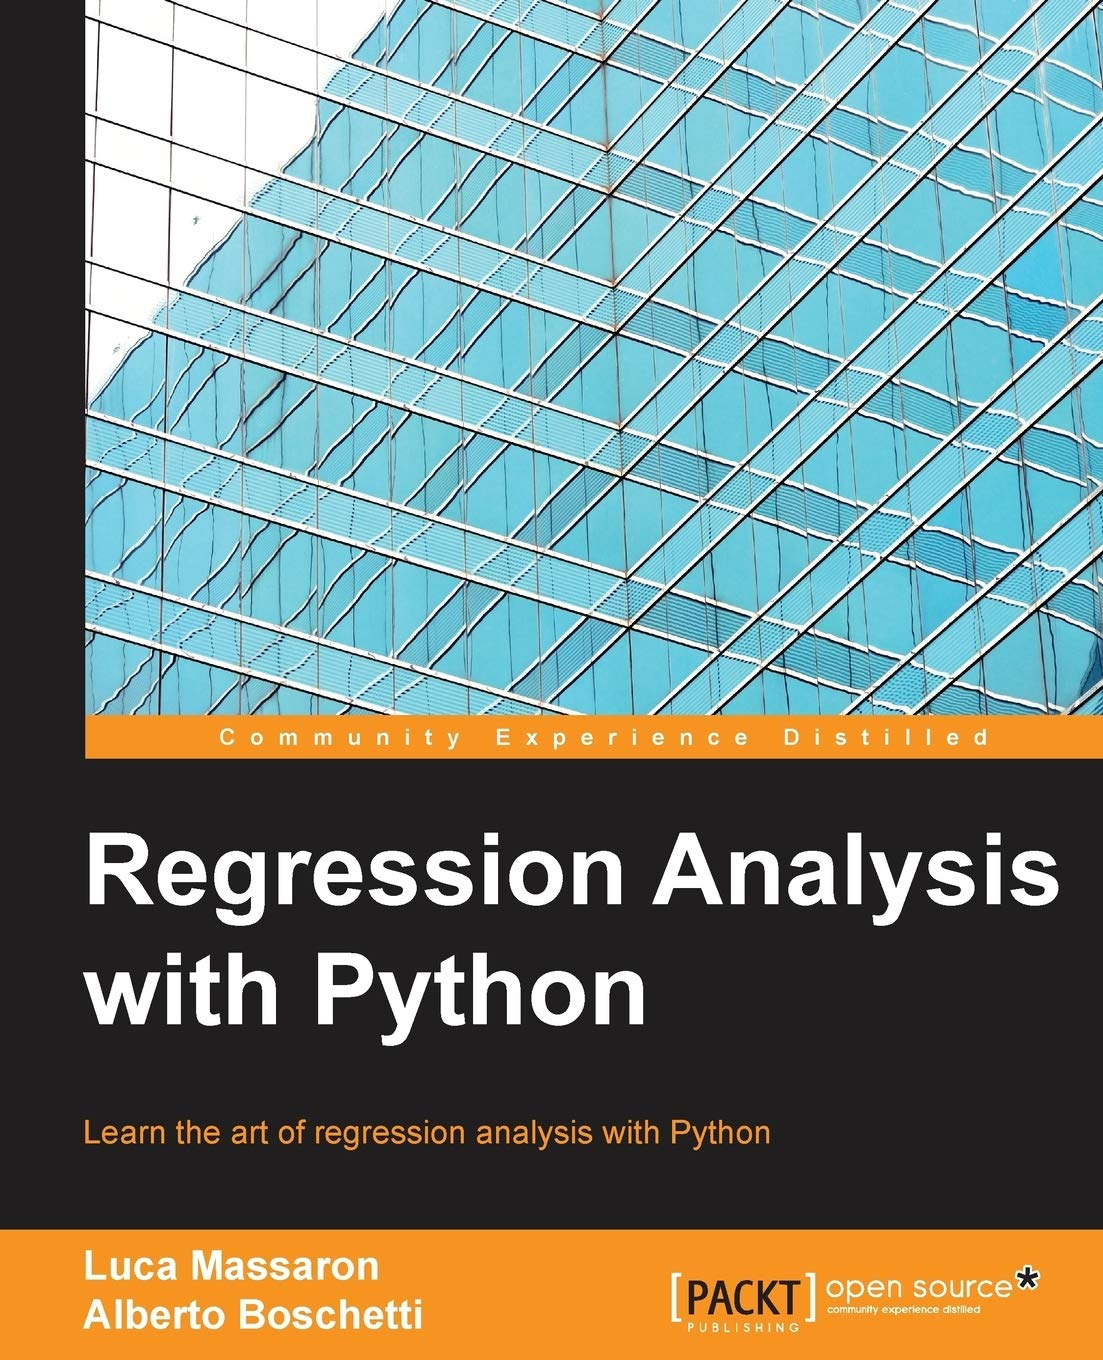
\includegraphics[width=.3\textwidth]{book2.jpg}
\end{figure}
El libro de \citeauthor{Massaron2016} \citeyear{Massaron2016} es un buen recurso para aprender a implementar análisis de regresiones. Esta aproximación es más orientada a machine learning, pero no hace una covertura adecuada al problema del chequeo de supuestos en regresión.
\end{frame}

\begin{frame}{Recursos Bibliográficos}
\begin{figure}
\includegraphics[width=.3\textwidth]{book3.jpg}
\end{figure}
El libro de \citeauthor{VanderPlas2017} \citeyear{VanderPlas2017} aborda básicamente data manipulation, data visualization, y machine learning. Su covertura deja por fuera un montón de estadística estándar en psicología u otras ciencias sociales (e.g., psicometría, modelos de ecuaciones estructurales, redes).
\end{frame}

\begin{frame}{Recursos Bibliográficos}
\begin{figure}

\includegraphics[width=.7\textwidth]{statsmodels.png}
\end{figure}
El paper de \citeauthor{Seabold2010} \citeyear{Seabold2010} es probablemente, a la fecha, el recurso más orientado a estadística que puede encontrarse en Python.\\
Su documentación online está disponible en \textcolor{blue}{\url{https://www.statsmodels.org/}}
\end{frame}

\section{Regresión Simple en Python}
\begin{frame}{Regresión Simple en Python}
Regresión con Mínimos Cuadrados Ordinarios
\scriptsize
\begin{verbatim}
\textcolor{magenta}{import} numpy \textcolor{magenta}{as} np\\
\textcolor{magenta}{import} statsmodels.api \textcolor{magenta}{as} sm\\
spector\_data = sm.datasets.spector.load(as\_pandas=\textcolor{orange}{False})\\
spector\_data.exog = sm.add\_constant(spector\_data.exog, prepend=\textcolor{orange}{False})\\
mod = sm.OLS(spector\_data.endog, spector\_data.exog)\\
res = mod.fit()\\
print(res.summary())
\end{verbatim}
\end{frame}


\begin{frame}{Regresión Simple en Python}
Regresión con Cuadrados Ordinarios Ponderados\\
\scriptsize
\begin{verbatim}
\textcolor{magenta}{import} numpy \textcolor{magenta}{as} np\\
\textcolor{magenta}{import} statsmodels.api \textcolor{magenta}{as} sm\\
spector\_data = sm.datasets.spector.load(as\_pandas=\textcolor{orange}{False})\\
spector\_data.exog = sm.add\_constant(spector\_data.exog, prepend=\textcolor{orange}{False})\\
mod = sm.WLS(spector\_data.endog, spector\_data.exog)\\
res = mod.fit()\\
print(res.summary())
\end{verbatim}    
\end{frame}

\begin{frame}{Regresión Simple en Python}
\begin{figure}
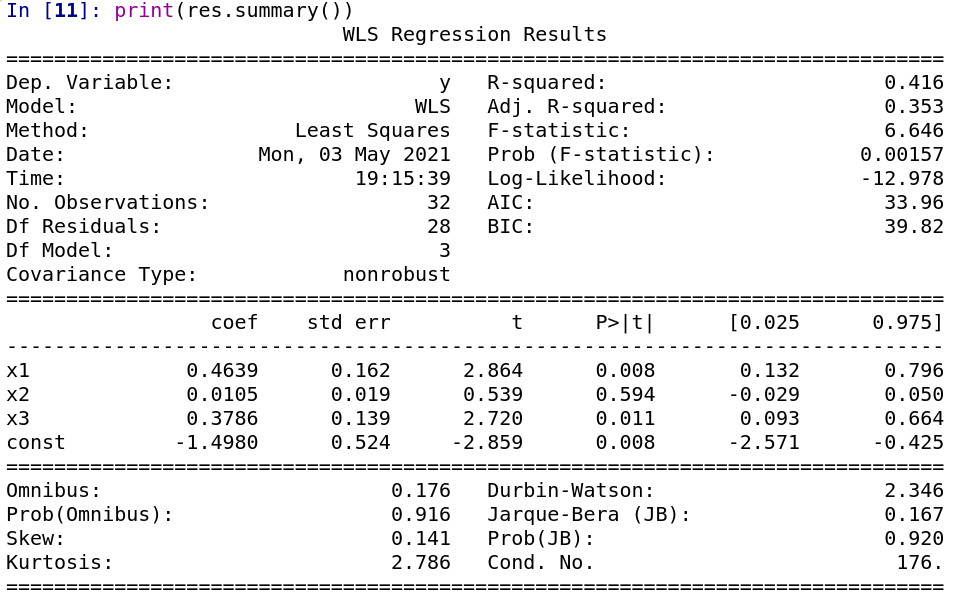
\includegraphics[width=.85\textwidth]{Output.png}
\end{figure}
\end{frame}

\section{Regresión Múltiple en Python}

\begin{frame}{Regresión Múltiple en Python}
\scriptsize
\begin{verbatim}
\textcolor{magenta}{import} pandas \textcolor{magenta}{as} pd\\
datos = pd.read\_csv(\textcolor{blue}{"/home/juan/cars.csv"})\\
\textcolor{magenta}{import} statsmodels.api as sm\\
\textcolor{magenta}{import} matplotlib.pyplot as plt\\
\textcolor{magenta}{import} statsmodels.formula.api as smf\\
results=smf.ols(\textcolor{blue}{'CO2 \~ ~ Weight + Volume'}, data=datos)\\
fitted\_model=results.fit()\\
fitted\_model.summary()
\end{verbatim}
\end{frame}

\begin{frame}{Regresión Múltiple en Python}
\begin{figure}
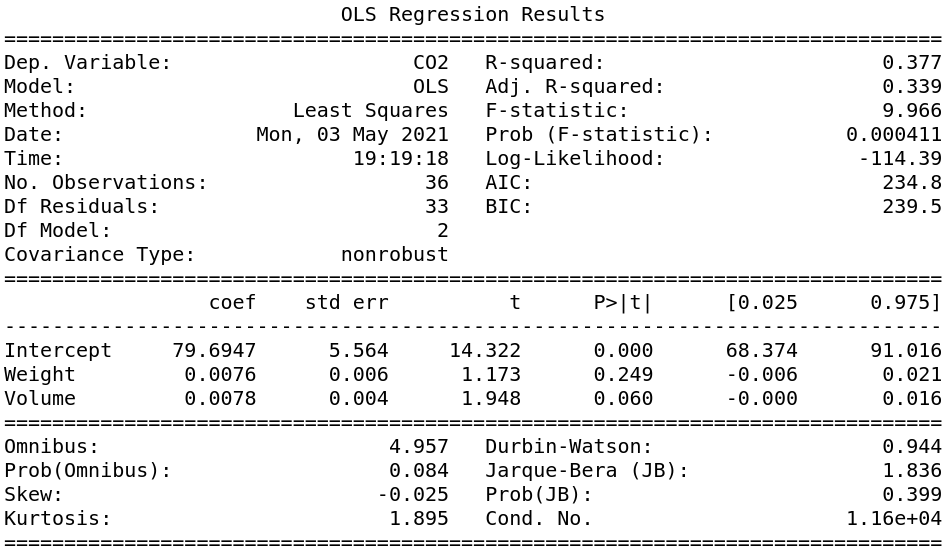
\includegraphics[width=.85\textwidth]{output2.png}
\end{figure}
\end{frame}

\begin{frame}{Regresión Múltiple en Python}
\scriptsize
\begin{verbatim}
fig = plt.figure(figsize=(8, 6))\\
results = smf.ols(\textcolor{blue}{'CO2 \~ ~ Weight + Volume'}, data=datos).fit()\\
sm.graphics.plot\_regress\_exog(results, \textcolor{blue}{'Volume'}, fig=fig)\\
plt.show()\\
\end{verbatim}
\begin{figure}
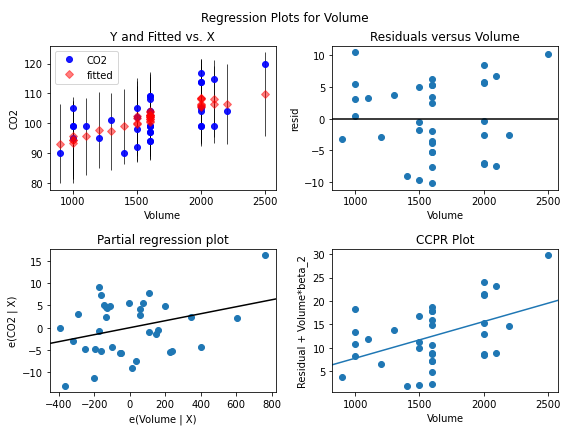
\includegraphics[width=.65\textwidth]{output3.png}
\end{figure}
\end{frame}

\begin{frame}[allowframebreaks]{Referencias}
\tiny
\bibliographystyle{apacite}
\bibliography{refs} 
\end{frame}

\end{document}